
%\begin{center}
%\begin{figure}[h]
%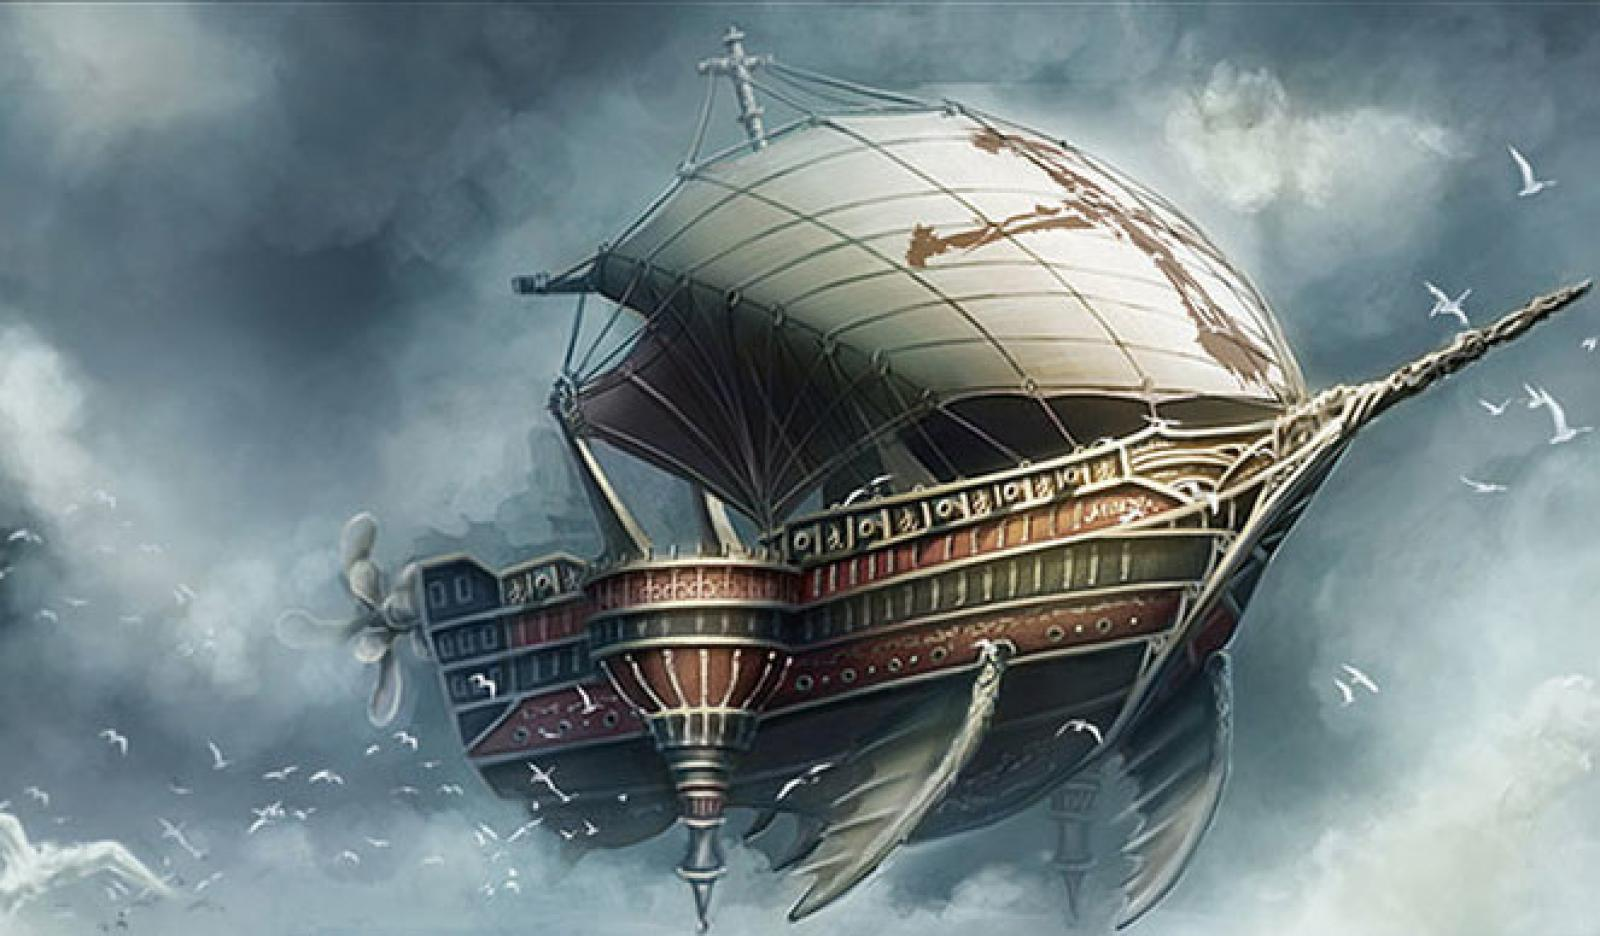
\includegraphics[width=60mm]{./content/img/theGary.jpg}
%\end{figure}
%\end{center}

\section{The Airship Gary}

\begin{multicols}{2}

\begin{center}
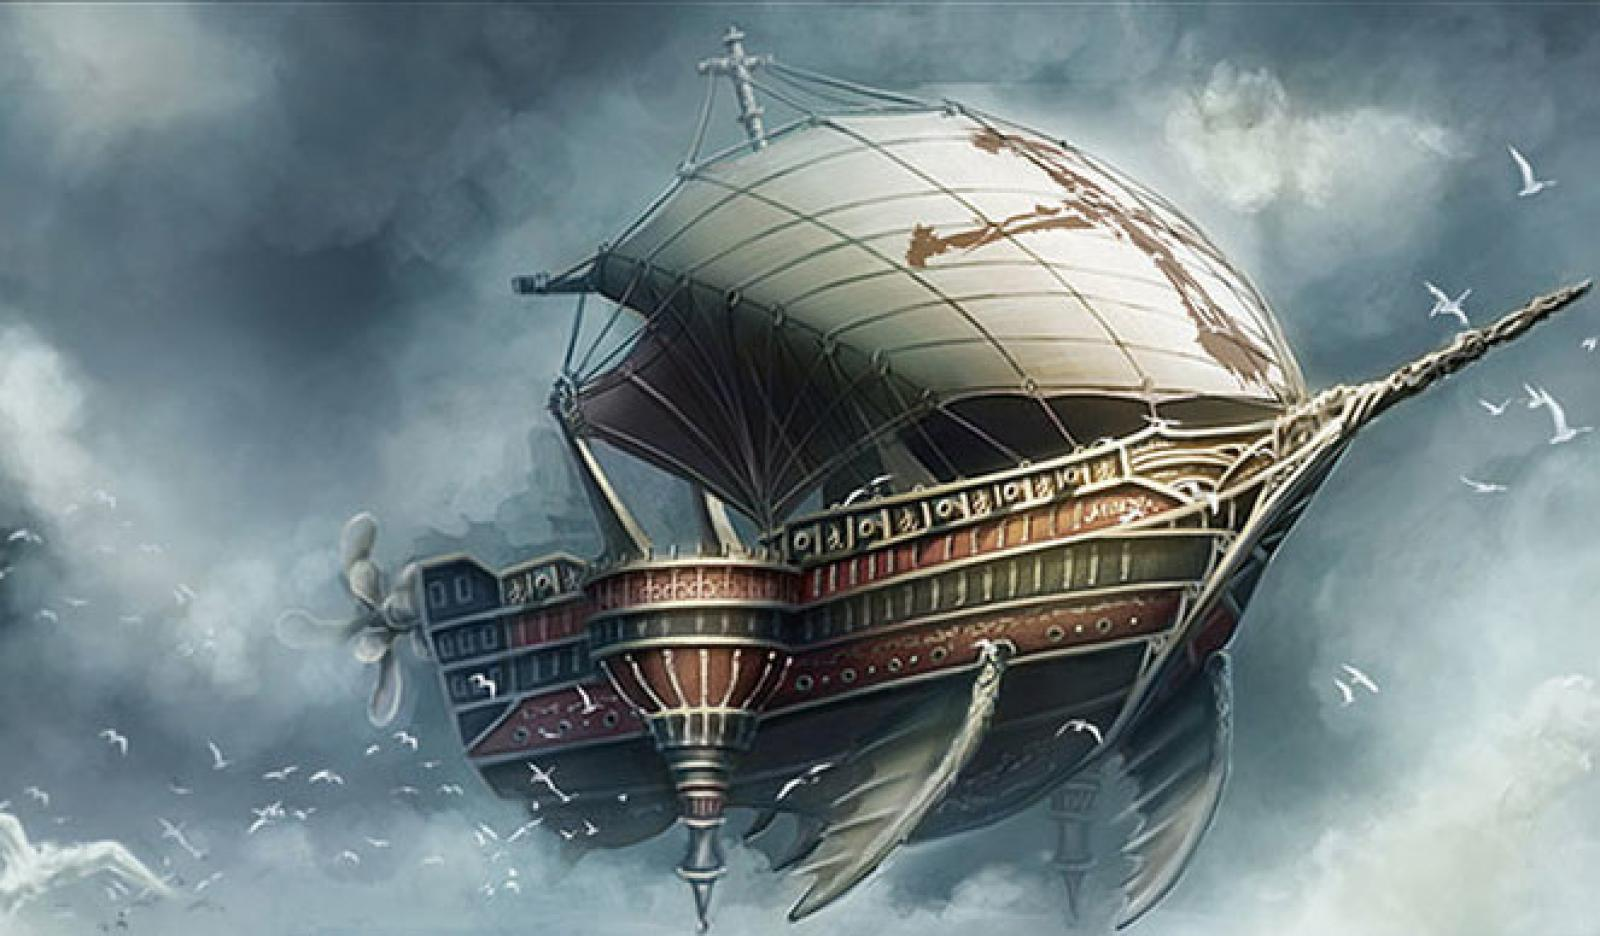
\includegraphics[width=80mm]{./content/img/theGary.jpg}
\begin{figure}[h]
\end{figure}
\end{center}

\subsubsection{Background}

The Good Airship Gary is the primary base of operations for the team.  The group discovered the airship within the Tower of Ruh'Breks, an ancient wizard's hidden stronghold buried deep underground.  Ruh'Breks himself, a dying sorcerer who had sealed himself away centuries ago, gifted the vessel to the party along with the legendary Puzzle Die.  The ship is powered by spectral energy batteries --- sentient ghost-like entities captured and contained within S.T.A.N.R.I's storage compartments.

Named after the group's beloved stone companion Gary, who sacrificed himself protecting the party in the jungles of South Africa, the airship became the symbol of the newly formed Gary Guild and the team's most prized possession.

The team have made a number of modifications to the ship over their time together, outfitting it with cannons, bomb bays, and an on-board workshop for Exme.  The latest major battle upgrade was completed during the campaign in Masuda, where gnomish engineers helped overhaul the ship's armaments in preparation for the assault on the Golden Hall.

\subsubsection{Functions}

The ship serves as mobile headquarters, offering sleeping quarters, Exme's engineering workshop, storage for the party's arsenal, and a command deck.  Its arsenal includes multiple cannons and a heavy forward-mounted weapon.  Captain Stick, a sentient wooden figurehead, has been entrusted with command of the vessel since its discovery.  S.T.A.N.R.I's on-board systems provide communications, navigation, and analytical support from the air.

\end{multicols}

\begin{center}
\begin{figure}[h]
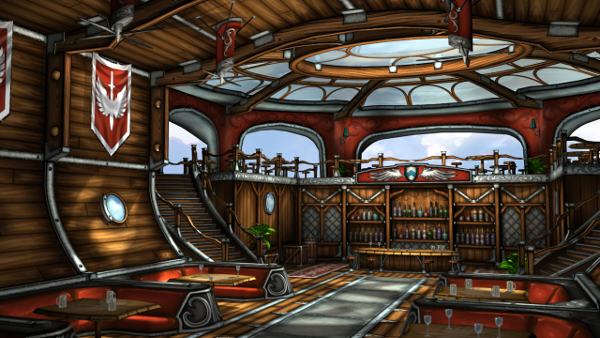
\includegraphics[width=\textwidth]{./content/img/theGaryInside.jpg}
\end{figure}
\end{center}

\clearpage

\vspace*{20mm}

\begin{center}
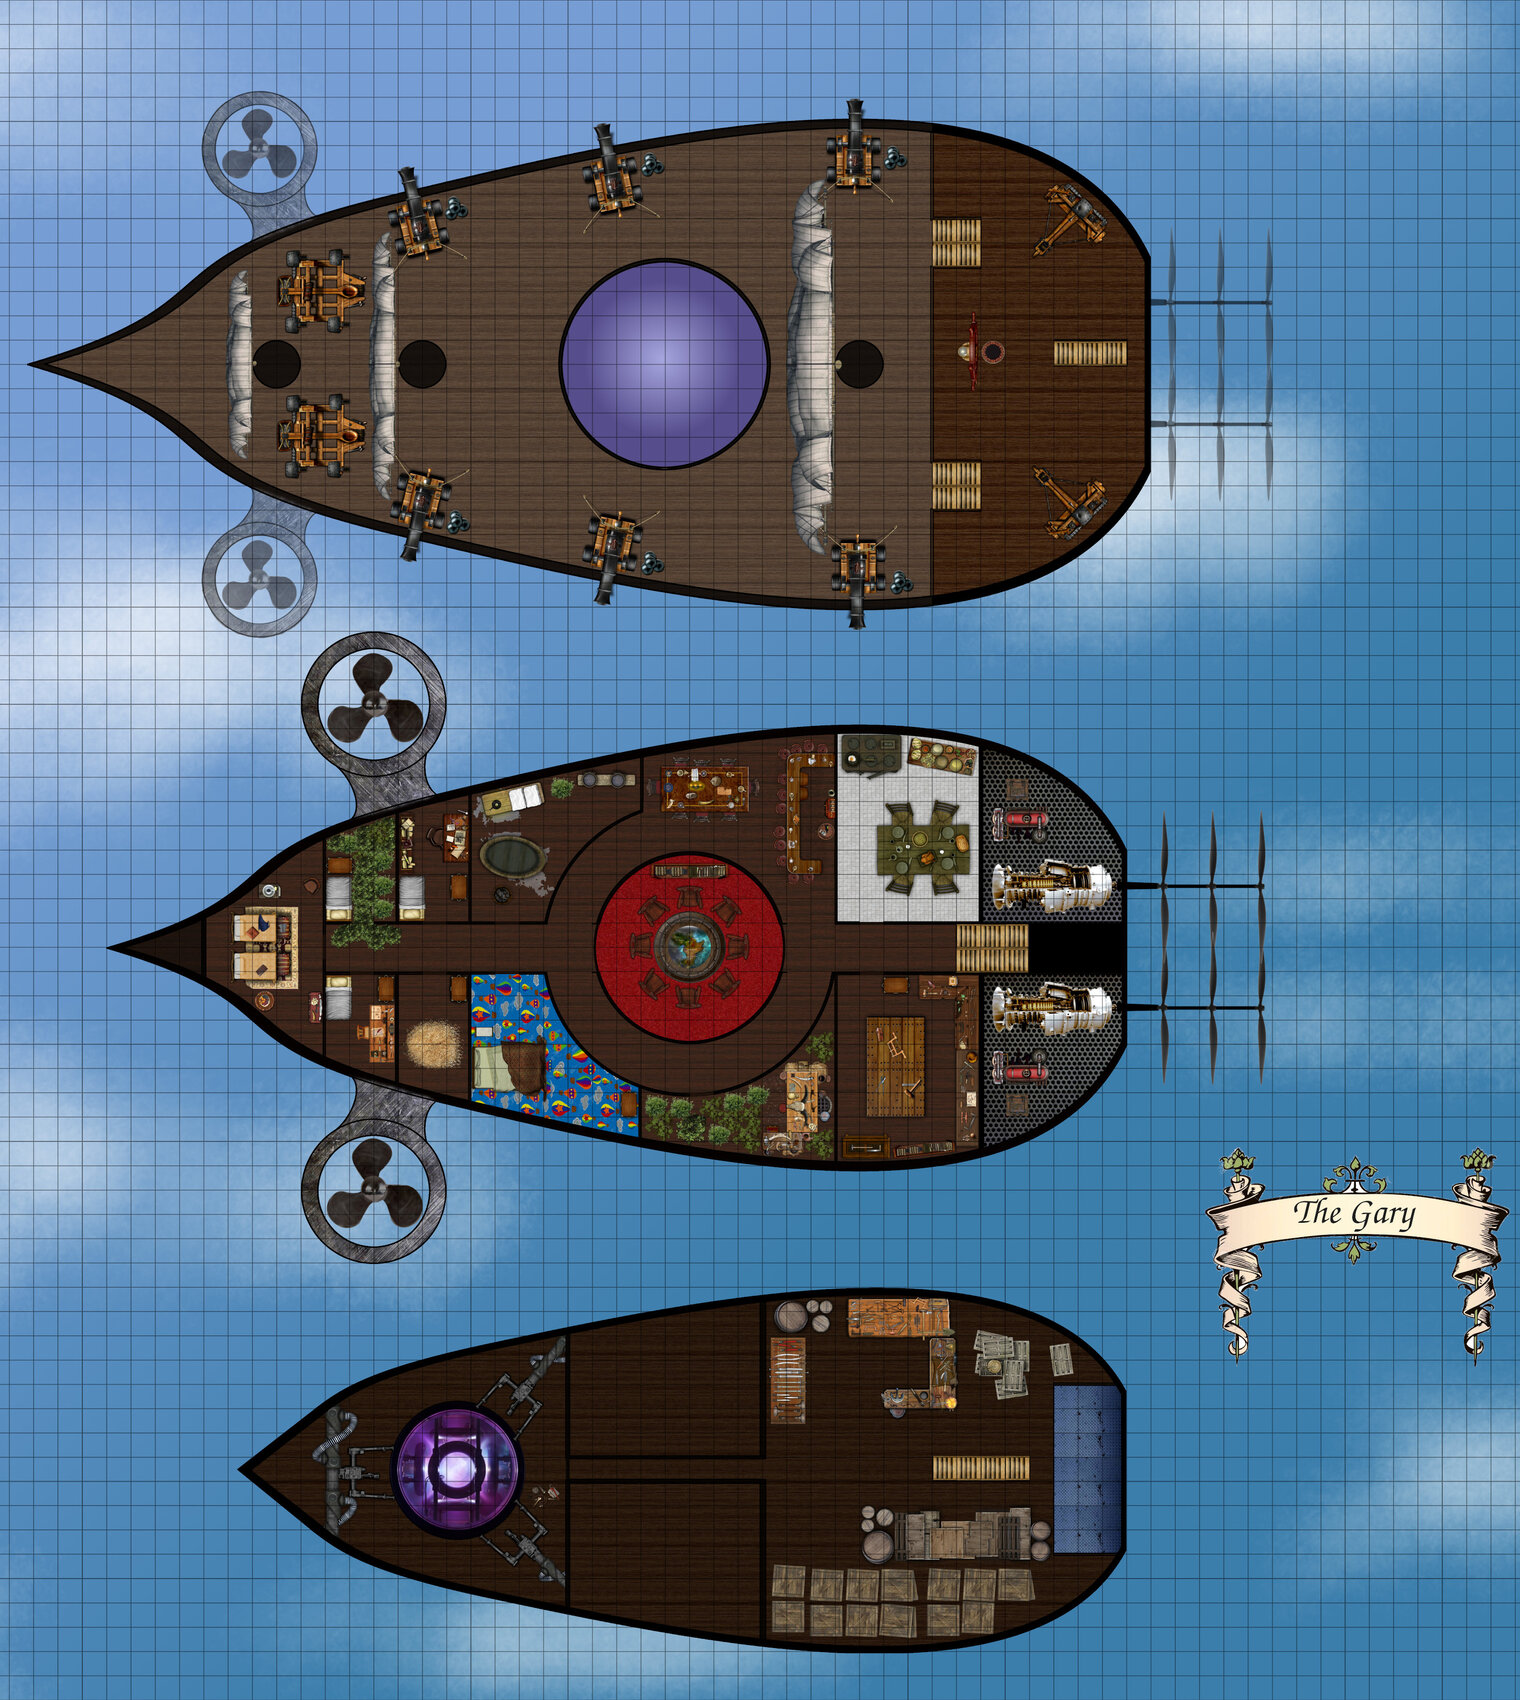
\includegraphics[width=180mm]{./content/img/theGaryMap.jpg}
\begin{figure}[h]
\end{figure}
\end{center}

\twocolumn

\clearpage